\subsection{Base de Datos SQLite}

\par \noindent
La base de datos SQLite definida en la sección es donde se guardan todas las medidas de temperatura realizadas por nuestro prototipo. El hecho de ser simplemente un fichero en nuestro smartphone lo hace versatil y efeciente para una base de datos local. 


\par \noindent
Por base de datos local hacemos entender que la información se mantendra en la memoria del smartphone que se este utilizando. SQLite se base en una base de datos SQL; por lo que, implementaremos una base de datos relacional. 

\begin{figure}[H]
	\centering
	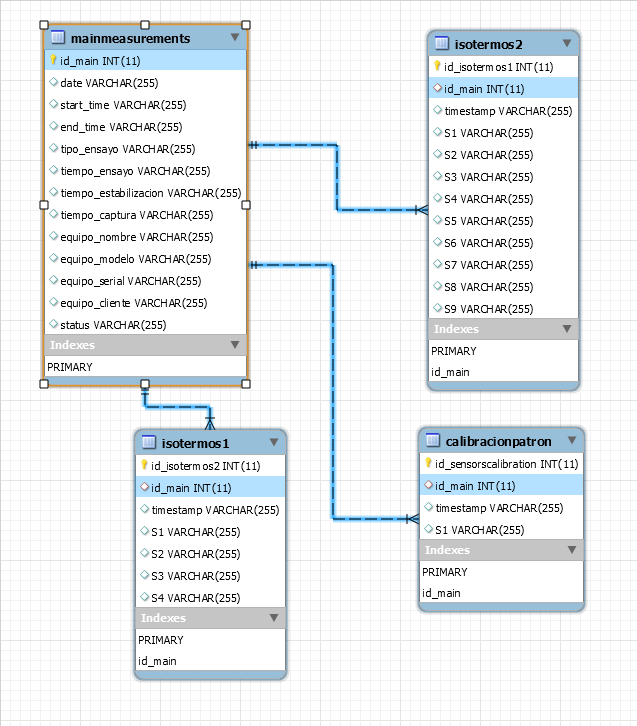
\includegraphics[width=0.8\linewidth]{db1.png}
	\caption{Estructura de la Base de Datos}
\end{figure}

\clearpage

\par \noindent
La tabla principal vendría siendo "mainmeasurements" donde se toman los datos del equipo y parámetros del ensayo. Mientras que las otra tablas con los nombres de los tipos de ensayo son donde se guardan las medidas de temperatura. Estas tablas estan relacionadas a la tabla principal, pero no entre ellas.


\par \noindent
Hasta el momento hemos cubierto el desarrollo del firmware del dispositivo, el código que maneja nuestro prototipo. La aplicación en android la cual guarda la información capturada por nuestro prototipo. El ultimo punto a cubrir es el armazón del prototipo. Recordemos que solamente hemos diseñado la placa del circuito. Para finalizar debemos diseñar el armazón, para diseñaremos un modelo tridimensional y lo imprimiremos utilizando una impresora 3D.

